\chapter{Background}
\label{chapter:background}

This chapter provides an overview of the main topics discussed in this thesis: namely, \emph{fuzzing} in Section~\ref{sec:whatIsFuzzing}, \emph{model-based testing} in Section~\ref{sec:whatIsModelBasedTesting}, \emph{mutation testing} in Section~\ref{sec:whatIsMutatinTesting} and \emph{delta-debugging} in Section~\ref{sec:whatIsDeltaDebugging}. Each section consists of a common definition of the corresponding topic, its terminology, techniques, typical workflow and its components. Furthermore, each section presents how the respective main topic is employed in this thesis and how these topics are related to each other.

\section{What Is Fuzzing?}
\label{sec:whatIsFuzzing}

\emph{Fuzz testing}, or simply \emph{fuzzing}, is a software testing technique which---in its original form introduced by Miller et al.~\cite{miller1995fuzz}---uses random generated data as input for the execution of software programs. The system under test, which can range from a single program to complex software infrastructure, is then monitored for unexpected behavior such as program crashes, and program defects, buffer overflows and memory leaks. Nowadays fuzzing is a popular choice for uncovering software vulnerabilities by security testing~\cite{mcnally2012fuzzing, sutton2007fuzzing, takanen2008fuzzing}, since it does not require to understand the source code or individual components of the system under test. Furthermore, fuzzing does not even require to have access to the source code but solely relies on the execution of the system. Hence, every generated input that exercises a problem during fuzzing, is a true positive for a deterministic system under test and therefore adds value to the testing process. This makes fuzzing, a superior choice in contrast to other techniques, at least if this characteristic is the most interesting for choosing a technique. For example static analysis, which looks at source code without executing it, relies on heuristics which can sometimes produce false positives. Hence, it can be necessary to check and verify every case manually, making such a technique far more inefficient.

The fundamental components of a fuzzer, the program for applying fuzzing, as described in~\cite{mcnally2012fuzzing}, are the \texttt{Fuzz Generator}, the \texttt{Delivery Mechanism} and the \texttt{Monitoring System}. These components, as well as their typical interactions, are depicted in Figure~\ref{fig:backgroundFuzzingFundamentalComponents}. The fuzz generator creates data which is then fed by the delivery mechanism to the system under test. Each system can have its own mechanism of accepting input data, e.g., a graphical user interface needs different actions than a program using a command line interface, and it is therefore the responsibility of the delivery mechanism to apply the correct actions for the given data and system. Observing the execution of these actions is the responsibility of the monitoring system that defines which problems can be found by the fuzzing process. The monitoring system can be as simple as checking the exit status of a program, i.e., to detect program crashes, or more sophisticated such as the instrumentation for buffer overflows during the execution of a program.

\begin{figure}[t]
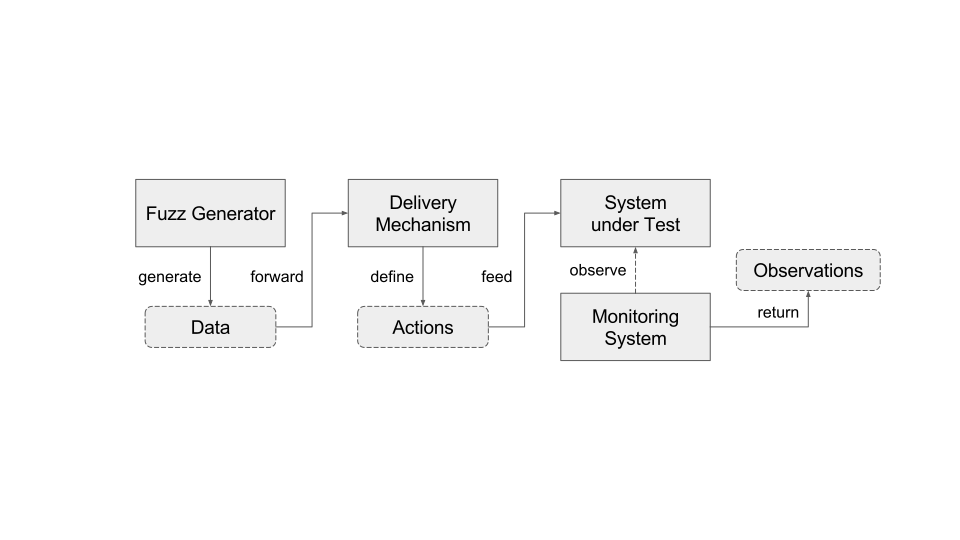
\includegraphics[width=1.0\textwidth]{images/background-fuzzing-fundamental-components.pdf}
\caption{Fundamental Components of Fuzzing}
\label{fig:backgroundFuzzingFundamentalComponents}
\end{figure}

Even though Miller et al.~showed in~\cite{miller1995fuzz} that the generation of random bytes as inputs for programs can harvest good results, its effectiveness gets limited by every conditional branch of the program under test. Each check and verification of a program requires the input data to be more structured for reaching deeper program areas. To overcome this issue two types of approaches are used by more advanced fuzz generators~\cite{takanen2008fuzzing}: \emph{mutation}-based and \emph{generation}-based techniques.

\subsection{Mutation-based fuzzing}
\label{subsec:mutatinFuzzing}

\emph{Mutation-based fuzzers}, or mutative fuzzers, take existing data and simply change it according to different rules. Such rules can be as simple as randomly toggling bits or as complex as combining two different sets of data into a new set. The advantage of mutation-based fuzzers is that they can work without the knowledge of how data must be structured and can therefore be implemented independently of the system under test. However, since they only adapt existing data, it is highly unlikely that program areas that are not bound to the existing data are exercised with the mutated data. Additionally, the advantage of using existing structured data is thwarted since the applied changes make the resulting data again more likely to be invalidated by existing checks and verifications of the program.

\subsection{Generation-based fuzzing}
\label{subsec:generationFuzzing}

\emph{Generation-based fuzzers}, or generative fuzzers, create new data without the need for existing data. They overcome the issues of mutation-based fuzzers by possessing an almost or even complete knowledge of the structure for the data that is valid for the system under test. By using this knowledge, which is called a model, data can be generated that exercises greater program coverage, since it complies to the expected structure and semantics of the system under test~\cite{miller2007analysis}.

Given that generative fuzzers have the knowledge of how valid data for a system under test has to be generated, they can be used as an efficient technique for positive testing. Hence, testing the system under test for expected behavior which includes valid as well as invalid data to test for expected error handling that is included in the specification. However, the knowledge of how valid data must be generated can also be used to derive invalid data by systematically adapting the underlying model to effectively apply negative testing. Hence, testing invalid cases which are not covered by the specification in order to provoke unexpected behavior such as system crashes.

Since one of the main goals of this thesis is to combine fuzzing and delta-debugging using the same underlying model, generative fuzzing seems to be the only logical choice for choosing an approach to implement fuzzing. However, generative fuzzing also has strong advantages over mutation-based fuzzing, such as not requiring to accumulate seemingly interesting test data, which can be a time-consuming task. Furthermore, generative fuzzing allows to accurately generate test data for specific scenarios while mutation-based fuzzing either requires to find such cases by chance or manually. An implementation of the generative fuzzing approach of this thesis can be found in Section~\ref{sec:fuzzingStrategies}. However, techniques rooted in mutation-based fuzzing can be applied to data models, thereby allowing effective negative testing in combination with mutation-based fuzzing. This exact combination has been implemented for this thesis and is described in Section~\ref{sec:fuzzingFilters}.

Even though fuzzing allows to effectively generate test data, it has the disadvantage of skipping one important part of testing software: verifying that specified requirements are implemented. In the subsequent section the software testing technique \emph{model-based testing} is introduced, which is able to fill this gap by requiring the validation of the system's output after feeding the system generated test data.

\section{What Is Model-Based Testing?}
\label{sec:whatIsModelBasedTesting}

\emph{Model-based testing} is a software testing technique which derives tests from a model that is based on the requirements on the system under tests. It is therefore a form of black-box testing. Furthermore, Utting et al.~define in \cite{utting2010practical} model-based testing to be \enquote{the automation of the design of black-box tests}, i.e., model-based testing does not only produce the input data for the execution of the system under test, but it must also generate executable test cases that include checks for the output of the system under test. An extensive list of case studies and references has been gathered by Utting et al.~in \cite{utting2010practical}, which showcase various benefits of model-based testing. Among them are reduced testing cost and time, as well as improved test quality, i.e., higher coverage of requirements testing.

The fundamental components of a model-based tester, according to~\cite{utting2010practical}, are the \texttt{Test Case Generator}, the \texttt{Test Script Generator} and the \texttt{Test Execution Tool}. These components, as well as their typical interactions, are depicted in Figure~\ref{fig:backgroundModelBasedTestingFundamentalComponents}. The test case generator uses the model to generate test cases for the system under test. These test cases may directly be executed. However, their form should be abstract in order to be able to reuse them in different environments. The test script generator then takes these test cases and transform them into test scripts which are either directly executable on the system under test, which is called online testing, or applicable using the test execution tool, which is called offline testing. The application of these test scripts outputs the final test results, i.e., whether a test case has passed the execution on the system under test.

\begin{figure}[t]
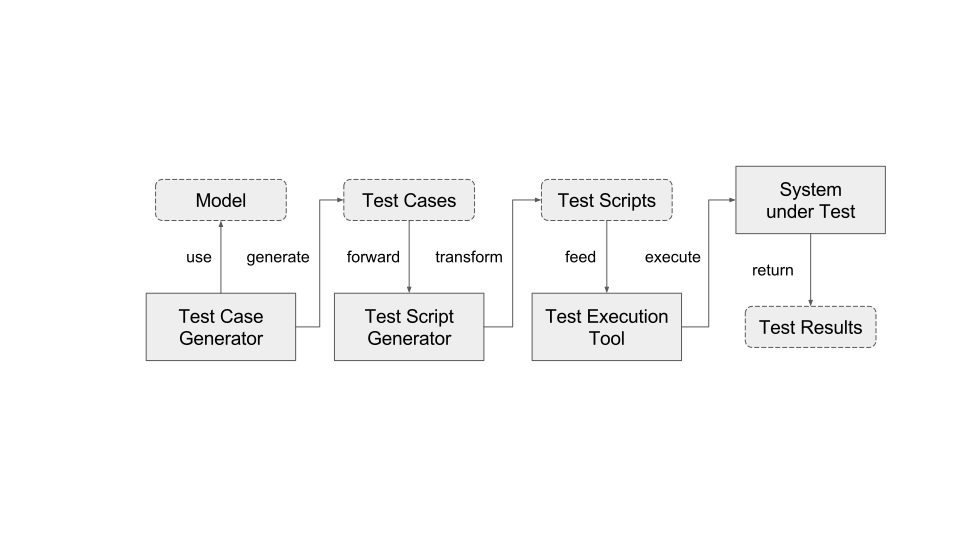
\includegraphics[width=1.0\textwidth]{images/background-modelbasedtesting-fundamental-components.pdf}
\caption{Fundamental Components of Model-based Testing}
\label{fig:backgroundModelBasedTestingFundamentalComponents}
\end{figure}

Model-based testing and generation-based fuzzing, as introduced in Section~\ref{sec:whatIsFuzzing}, utilize a data model to be able to derive and execute tests. Hence, it is only fitting to compare both techniques:
\begin{itemize}
\item The fuzz generator of the fuzzer has the same behaviors and responsibilities as the model and test case generator of a model-based tester.
\item The delivery mechanism of the fuzzer has the same behaviors and responsibilities as the test script generator and the test execution tool of the model-based tester.
\item The online testing variant of model-based testing can also be directly compared to feedback-driven fuzzing. Both techniques executed their cases directly on the system and require some kind of monitoring of the system under test. The feedback of the monitoring can then be incorporated into the test cases, e.g., to check if an error message occurred, and guide the generation of the next test case.
\end{itemize}
Even though we can directly compare generation-based fuzzing to model-based testing, we can also observe three major differences: Model-based testing is much stricter concerning the model which is used to generate test cases. It has to be based on the requirements of the system under test. Furthermore, the validation of the system's output, which is a requirement for model-based testing, is not necessary for a fuzzer, but can be adopted by the monitoring system. Lastly, model-based testing strives to generate reusable test cases which are semi-executable, while fuzzing is often described of only generating inputs which can be used as parameters for test cases or the execution of the system under test.

These differences make model-based testing an attractive addition to fuzzing to completely cover the whole spectrum of software testing. As a result, this thesis introduces with the \textsc{Tavor framework} in Chapter~\ref{chapter:tavorFramework} and the \textsc{Tavor format} in Chapter~\ref{chapter:tavorFormat} capabilities to define and structure functional test cases which include the validation of requirements. Furthermore, Chapter~\ref{chapter:tavorCLI} introduces with the \textsc{Tavor CLI} functionality to communicate with the systems under test. These additions allow the utilization of model-based testing which are showcased in the evaluation presented in Chapter~\ref{chapter:evaluation}.

Since both, fuzzing and model-based testing, allow to generate test cases to form test suites, a suitable method for evaluating these test suites must be employed. The subsequent section introduces \emph{mutation testing}, which allows to measure the effectiveness of a test suite to detect faults in the system under test.

\section{What Is Mutation Testing?}
\label{sec:whatIsMutatinTesting}

\emph{Mutation testing} is, according to an extensive survey by Jia et al.~\cite{jia2011analysis}, a \enquote{fault-based testing technique which can be used to measure the effectiveness of a test set in terms of its ability to detect faults}. The technique introduces faults, which are represented as syntactical changes to the program's binary or source code called \emph{mutations}, to create faulty programs named \emph{mutants}. Each mutant is then tested by executing an existing test set of the program. If the result of running the test set with the mutant differs from the result of running the test set with the original fault-free program, then the mutant has been killed, i.e., it has been detected by the test set. If the mutant has not been killed, either the test set needs to be extended to detect the modification or the mutant is equal to the original program. The effectiveness of the test set can then be calculated by the number of killed mutants by the total amount of tested mutants. This metric is called the \emph{mutation score} which can be used to directly compare two distinct test sets for the same program. Hence it can, for instance, be used to compare handwritten to automatically generated test sets of programs. A mutation score of $1.0$ is most desirable since this means that a test set killed all mutations.

Significant to the field of mutation testing are two hypothesis defined by DeMillo et al.~\cite{demillo1978hints}: the \emph{Competent Programmer Hypothesis} and the \emph{Coupling Effect}. They imply that it should be sufficient to examine only a subset of simple faults of the overall possible program faults, to be effective in finding real faults~\cite{jia2011analysis}.
\begin{itemize}
\item The \emph{Competent Programmer Hypothesis} states that \enquote{programmers are competent, which implies that they tend to develop programs close to the correct version}~\cite{jia2011analysis}. It can be therefore assumed that the existing faults in a program are simple. Therefore, it is sufficient to introduce simple faults by mutation testing because it mimics the faults that are made by competent programmers.
\item The \emph{Coupling Effect} states that \enquote{test data that distinguishes all programs differing from a correct one by only simple errors is so sensitive that it also implicitly distinguishes more complex errors} \cite{demillo1978hints}. Therefore, it is sufficient to examine only simple errors since they are coupled with complex errors in the program under test.
\end{itemize}

The fundamental components of mutation testing can be derived from the traditional process described in~\cite{demillo1978hints, jia2011analysis}, namely: the list of \texttt{Mutation Operators} to apply modifications and a \texttt{Test Set} of the program under test. These components, as well as their typical interactions, are depicted in Figure~\ref{fig:backgroundMutationTestingFundamentalComponents}. First the original program $P$ is executed against the test set $T$, producing the test result $R$. Then each mutation operator $M$ takes the original program under test $P$ and applies its modifications. The outcome is a set of modified programs $P'$, the so called mutants. These modified programs $P'$ are then executed against the test set $T$. The produced test results $R'$ of this step are compared to the original test result $R$. If the results are equal, the mutant $P'$, and therefore its modifications, has not been detected by the test set $T$.

\begin{figure}[t]
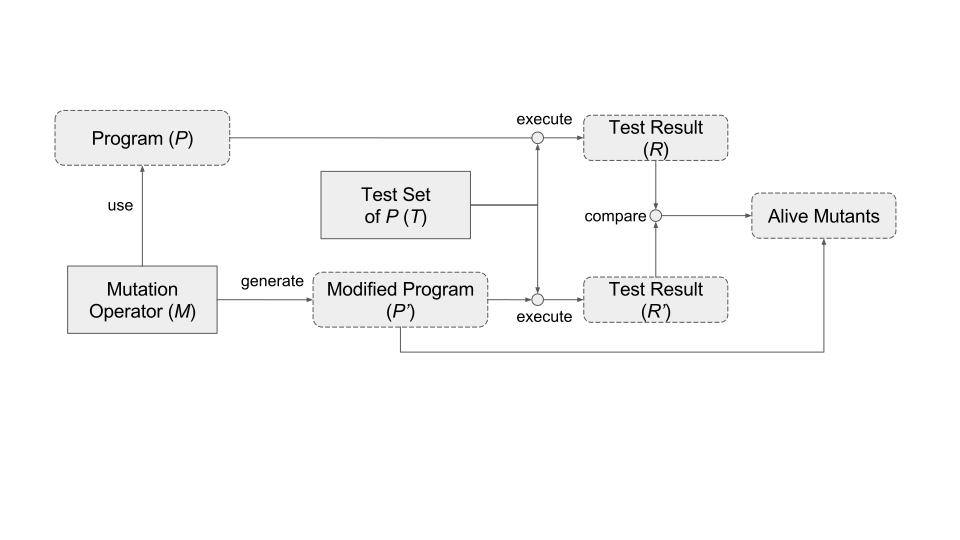
\includegraphics[width=1.0\textwidth]{images/background-mutationtesting-fundamental-components.pdf}
\caption{Fundamental Components of Mutation Testing}
\label{fig:backgroundMutationTestingFundamentalComponents}
\end{figure}

Although the definition of mutation testing states that it is applied to detect faults in programs, it can also be used to uncover implementation flaws such as dead code. Furthermore, mutation testing is mostly described to solely cover techniques for program source code. However, it has also been used to mutate program specifications~\cite{jia2011analysis}. The latter direction is called \emph{specification mutation}, which is a black-box or grey-box testing technique depending on what program parts are used, while the first direction is called \emph{program mutation} which solely focuses on the program binary or source code and is therefore a white-box testing technique~\cite{jia2011analysis}.

This thesis utilizes mutation testing in Chapter~\ref{chapter:evaluation} to evaluate the effectiveness of generated test suites. The direction of program mutation is used, to emphasize how much of the system under test is actually covered. Since everything that has been implemented for this thesis is written in the programming language \textsc{Go}, it is only fitting to include in the evaluation of this thesis at least one scenario of a \textsc{Go} program. Chapter~\ref{chapter:goMutesting} introduces \textsc{go-mutesting} to perform the mutation testing part for the evaluation of the mentioned scenario.

Determining the effectiveness of test suites is just one discipline that needs to be considered while generating test cases. Another discipline arises when individual test cases are executed. The execution of a test case either verifies that the system under test behaves as defined by the test case, or the test case fails which highlights a fault that must be investigated. One possible method to aid in the time-consuming and complicated process of investigating and patching faults is the reduction of failing test cases. The subsequent section introduces \emph{delta-debugging}, an automatic technique to systematically reduce data such as test cases.

\section{What Is Delta-Debugging?}
\label{sec:whatIsDeltaDebugging}

\emph{Delta-debugging} is defined by Zeller in~\cite{zeller2009programs} as an \enquote{automatic technique that narrows down a cause by running automated experiments}. The typical use case is the reduction of input data which lets a program fail during execution. Less data has the benefit of having to consider less context during debugging a problem. Therefore, delta-debugging makes it possible for the user to focus only on relevant parts of the failure-inducing data. Note that finding the minimal representation, which still provokes the same program behavior of the original data, is not guaranteed by process of delta-debugging~\cite{brummayer2009fuzzing, brummayer2010automated}. However, in practice every reduction of the context that is needed to debug a problem is already an improvement. Furthermore, delta-debugging can be used to reduce and isolate anything, given appropriate implementations of the delta-debugging phases. For instance a solution might be reduced to be more readable or a huge formula is rewritten to a smaller formula which has the same behavior.

The fundamental components of a delta-debugger, which can be derived from the original algorithm~\cite{zeller2009programs}, are the \texttt{Reduction Algorithm} and the \texttt{System Under Test}. These components, as well as their typical interactions, are depicted in Figure~\ref{fig:backgroundDeltaDebuggingFundamentalComponents}. First the original data $D$ is executed with the system under test. The resulting execution determines the original behavior $B$ which must be preserved during the reduction. Next the original data $D$ is fed into the reduction algorithm. The algorithm determines which parts of the data should be reduced for the current reduction iteration, and how the selected part is reduced, i.e., removed or substituted. The reduced data $D'$ is then executed with the system under test. The resulting behavior of the execution $B'$ is compared to the behavior of the execution with the original data $B$. The result of this comparison is fed back into the reduction algorithm. If both behaviors are the same, the original behavior got preserved and the reduction algorithm continues with the next reduction iteration. Otherwise the last reduction is reverted and the algorithm proceeds. This reduction loop continues until predefined conditions are met, e.g., a timeout occurs or the algorithm does not find new parts to reduce.

\begin{figure}[t]
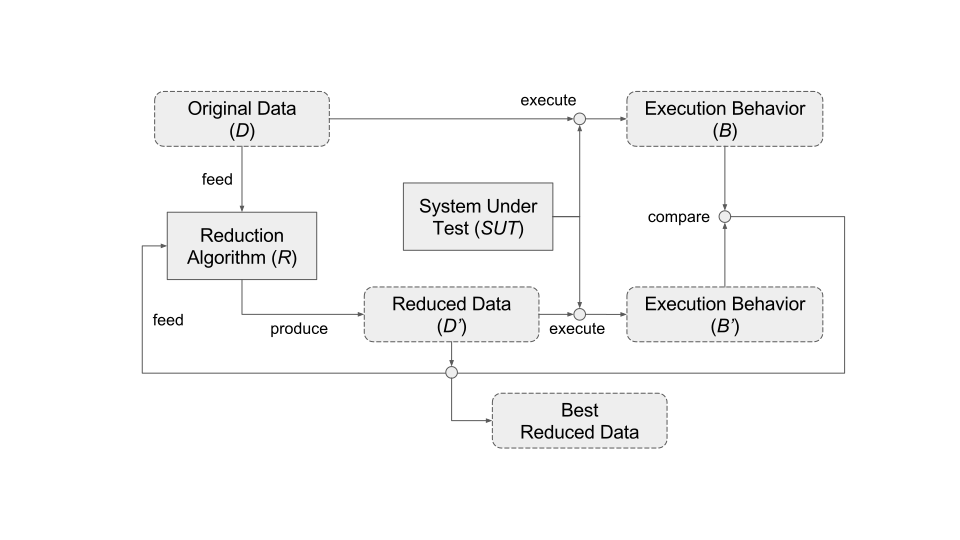
\includegraphics[width=1.0\textwidth]{images/background-deltadebugging-fundamental-components.pdf}
\caption{Fundamental Components of Delta-Debugging}
\label{fig:backgroundDeltaDebuggingFundamentalComponents}
\end{figure}

Considering the main components and workflow of delta-debugging, we can define the following three phases:

\begin{itemize}
\item The \emph{search phase} decides which part of the data will be reduced next.
\item The \emph{reduction phase} removes repetitions and optional data or replaces data with something else, e.g., uninteresting complex functions are replaced with constant values.
\item The \emph{testing phase} checks if the reduced data still provokes the original failure.
\end{itemize}

The original delta-debugging algorithm~\cite{zeller2009programs} reduces the given data at the character level, ignoring the syntactical structure of the data. Hence, making it likely to produce invalid data, leading to a high amount of rejected reduction iterations. By making the search phase aware of the data's structure an immense reduction in iterations can be achieved, dramatically speeding up the delta-debugging process~\cite{misherghi2006hdd, brummayer2009fuzzing, brummayer2010automated}. Additionally, making the reduction phase aware of the content itself, can be very efficient in reducing the original data greatly while also reducing the runtime of the process~\cite{brummayer2009fuzzing, brummayer2010automated}.

Making the delta-debugging implementation aware of the data's structure and content, basically giving the implementation an almost or even complete model of the provided data, is one of the goals of this thesis. Section~\ref{sec:reducingStrategies} describes the approach and implementation which completes the goal of combining fuzzing and delta-debugging by utilizing the same underlying model.
